\begin{frame}{Introduction (1): What is version control?}
  \begin{columns}[onlytextwidth]
    \begin{column}{0.6\textwidth}
      \begin{itemize}
          \item tracks any kind of content
            \inote{e.g. websites, software, presentations}
          \item knows about different versions
          \begin{itemize}
            \item knows what was changed when
            \item can revert changes if something goes wrong
          \end{itemize}
          \item has a collaboration component
          \begin{itemize}
            \item several people can work together on the same project
            \item changes can be synced
            \item easy to see who changed what
          \end{itemize}
        \end{itemize}
    \end{column}
    \begin{column}[t]{0.4\textwidth}
      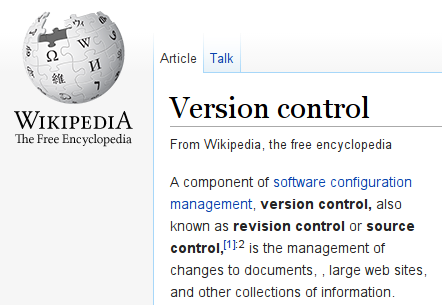
\includegraphics[width=0.95\textwidth]{imgs/vc_wikipedia}
    \end{column}
  \end{columns}
\end{frame}

\begin{frame}{Introduction (2): What is git and why use it?}
  \begin{columns}[onlytextwidth]
    \begin{column}{0.6\textwidth}
      \begin{itemize}
        \item git -- ``the stupid content tracker''
        \begin{itemize}
          \item open-source version control system
          \item fast, scalable, distributable
        \end{itemize}
        \item originally developed in 2005 for maintaining the linux kernel source code
      \end{itemize}
    \end{column}
    \begin{column}[t]{0.4\textwidth}
      
\includegraphics[width=0.95\textwidth]{imgs/git_logo}
    \end{column}
  \end{columns}
\end{frame}

\begin{frame}{Introduction (3): What is git and why use it?}
  \begin{itemize}
    \item git is both for beginners and advanced users
    \begin{itemize}
      \item provides high-level-commands
      \item additonally gives full access to internals
    \end{itemize}
    \item git is distributed - and it is easy to sync changes
    \begin{itemize}
      \item no central server to share content required
      \item changes can be synced in many ways
      \item http(s), ssh, git protocol, diffs via email, \dots
    \end{itemize}
  \end{itemize}
\end{frame}